\chapter{Artificial Neural Networks (ANNs)}\label{chap:ann}
This chapter will discuss the basics of artificial neural networks (ANNs) which will be referenced throughout the rest of the thesis. All the techniques and theory discussed in this chapter have been used in some way to achieve the results presented in chapter \ref{chap:results}. This chapter will not introduce anything new to someone who is familiar with ANN.

\section{Introduction to ANN}
An artificial neural network is a machine learning model inspired by biological neural networks \parencite{lippmann1987introduction}.  Goodfellow and colleagues (2016) describes an ANN as a directed and acyclic graph (see figure \ref{fig:simple_ann}). They go on to say that the network is constructed of artificial neurons which are structured in layers -- these neurons are represented as nodes in a graph. Each neuron represents a function that takes some input from other nodes and produces an output. The input data to the network is represented by a vector $\vec{x}$ with $n$ features, as shown in equation \ref{eq:input_vec}. The vector $\vec{x}$ could for example represent a whole sentence where $x_i$ represents a word.
\begin{equation}\label{eq:input_vec}
    \vec{x} = [x_1, x_2, x_3, \dots , x_n]^T
\end{equation}
The edges in the network are connections between pairs of neurons. Each connection between two neurons have a weight. These weights will change as the network is optimised, as described in section \ref{sec:trainingoptimisation}, and the way they change will directly change the networks output. Updating the weights between neurons is a key part of how an ANN works, as the connections directly affect the output of the network. In practice this means that the weights should be updated so that the network iterativly produces a output that is becomes more smilirar to the target. 
\\\\
The input to a layer is the matrix product between the output from a previous layer and the weights between those two layers (usually also with some bias term added). The weights are used to transform the input before it is propagated to subsequent layers. A convenient way to represent weights between two layers $j$ and $k$ is by a matrix, $W_{jk}$, where each element is the weight between a neuron in layer $k$ and a neuron in layer $j$, where $k<j$. Let $\vec{z_j}$ denote the input to layer $j$ where $W_{jk}$ are weights to layer $j$ from layer $k$ and $\vec{x_k}$ is the output from layer $k$. The vector $\vec{b}$ is a bias term that is added for more degrees of freedom. 
\begin{equation}\label{eq:z}
    \vec{z_j} = \vec{W_{jk}} \cdot \vec{x_k} + \vec{b_j}
\end{equation}
Let $\vec{y_i}$ denote the output of the layer $i$. For the first layer (input layer) $\vec{y_1}=\vec{x}$. The output, $\vec{y_i}$, of a layer $i$ is the result of applying some activation function on $\vec{z_i}$ as shown in equation \ref{eq:f_of_z}. Activation functions are described in further detail in section \ref{activationfunction} but can in summary be seen as a way to scale the output.
\begin{equation}\label{eq:f_of_z}
    \vec{y_i} = f(z_i)
\end{equation}
Once the data has been propagated to the last layer, an error function will be used to measure the error of the model by comparing the final output/prediction with the expected output for the given input. The details about error functions can be found in section \ref{errorfunction}. Furthermore, the results of the error functions are used when training the network, which is explained in section \ref{sec:trainingoptimisation}. 
\\\\
Depth and width are often used to describe the shape of an artificial neural network \parencite{Goodfellow-et-al-2016}. The depth determines how many layers the network contains. The layers between input and output layer are called hidden layers. The more neurons a layer have the wider it is considered. \parencite{Goodfellow-et-al-2016} states that the reason for using multiple layers are taken from research in neuroscience. A large network (in either dimension) has more degrees of freedom which generally means that it will fit the data better, but will possibly overfit (see section \ref{sec:overfitting}).

\begin{figure}[h]
    \centering
    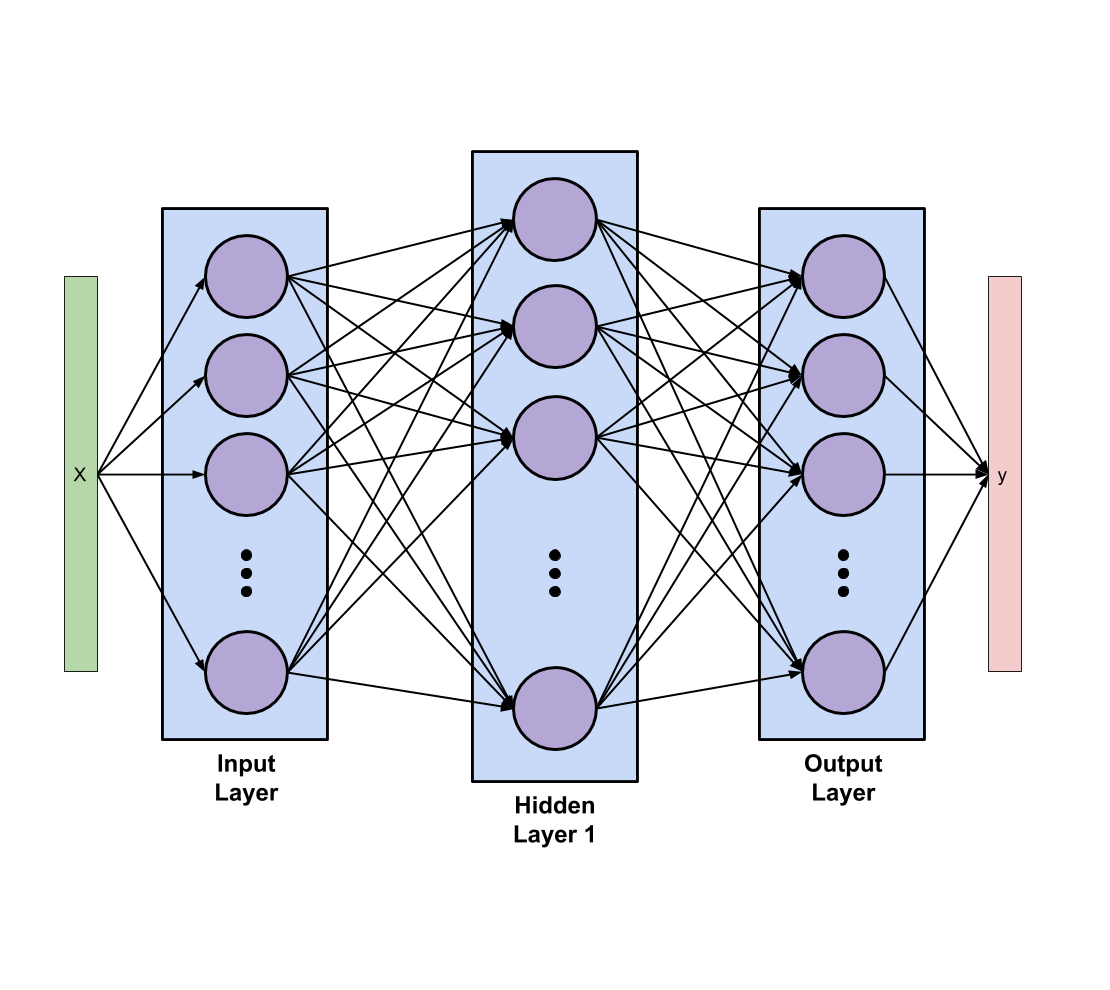
\includegraphics[width=0.75\textwidth]{figure/ann/simple_ann}
    \caption{A graph visualisation of a simple ANN. $\vec{x}$ and $\vec{y}$ are input and output vectors respectively}
    \label{fig:simple_ann}
\end{figure}

\section{Uses of ANN}
A common use of machine learning is classification. It is the task of classifying a given data point as belonging to one (or more) of $k$ sets based of previously observed data \parencite{Michie94machinelearning}. Classification can be visualised as a graph of data points with a curve separating the $k$ sets, this curve is also referred to as decision boundary. For the purpose of this project an artificial neural network will be used for classifying content to users. There are however a lot of different machine learning techniques which solves the problem of automatically classifying data, e.g. Naïve Bayes classifier \parencite{rish2001empirical}, Support Vector Machine (SVM) \parencite{boser1992training, cortes1995support}, or Decision Trees \parencite{source}.
\\\\
Classification of data typically requires extraction of features that can be compared - feature engineering, as this is called, is a manual process that usually requires extensive domain knowledge. When using artificial neural networks, the process of feature engineering can be omitted  thus making it easier to model more complex problems \parencite{nlp2011ronan, lecun2015deep}. This ability of artificial neural networks makes them suitable to model sequences of text as it is not necessary to manually find features in the text that could be used for classification, which motivates their usage for this project.


\section{Activation functions}\label{activationfunction}
The activation function scales the output from a node to create a new signal that is sent to the next layer \parencite{basheer2000artificial}. By using non-linear functions it is possible to scale the output, and find non-linear decision boundaries which allow better fitting to the data \parencite{lippmann1987introduction, basheer2000artificial}. Different activation functions can be used for different purposes in the same artificial neural network, it is not necessary to choose only one. In this project a few different activation functions have been used, and are described below.

\subsection{Logistic function}\label{sec:sigmoid_function}
The logistic function is a non-linear function with a sigmoid curve defined by equation \ref{eq:sigmoid} that squashes the input, $z_j$ from equation \ref{eq:z}, between $[0, 1]$. A sigmoid function is a function with an \textit{S} shape, another sigmoid functions is $tanh(\vec{x})$ which is used in lstm \ref{sec:rnn}.
\begin{equation}\label{eq:sigmoid}
    f(\vec{x})=\frac{1}{1+exp(\vec{-x})}
\end{equation}
For this project the logistic function has been used in the final layer as the output function as it is possible to interpret its output as probabilities. This particular function is especially useful for multi-label classifications (where some input can be classified as belonging to more than one class, like the problem presented in this thesis). When using the logistic function like this it is common to use the negative log-likelihood error function as this is particularly useful for multi-label classifications \parencite{bishop1995neural}.

\subsection{Rectified Linear Unit (ReLU) function}\label{sec:relu}
The ReLU function is a non-linear function defined by equation \ref{eq:ReLU}. This function has the benefit of being unbounded as opposed to the logistic function, the range of which is the interval $[0, 1]$. The ReLU function has become popular in the past few years due to it being less susceptible to vanishing gradient compared to other activation functions \parencite{glorot2011deep, lecun2015deep}.
\begin{equation}\label{eq:ReLU}
    f(x) = max(0,x)
\end{equation}
The ReLU function was used as the activation function in the hidden layers.

\subsection{Softmax function}\label{sec:softmax_function}
The softmax function is defined by equation \ref{eq:softmax} where $\vec{x}$ is a vector of $n$ outputs. Softmax scales the vector entries to be between $[0,1]$, while normalising them all to sum to 1.
\begin{equation} \label{eq:softmax}
    f(x_j) = \frac{e^{\vec{x}_j}}{\sum_{i=1}^{n} e^{\vec{x}_i}}
\end{equation}
When using the softmax function in the final layer of the network to create an output it has been shown that the cross entropy error function gives a better accuracy compared to others \parencite{dunne1997pairing,golik2013cross}. By using the softmax activation function the output can be interpreted as normalised probabilities between the $n$ output classes. Because of the normalisation this becomes useful for classification where there is only one correct true class. Softmax is used during pretraining of the network, when it is trained to predict exactly one subreddit. (see section \ref{sect:enhacing_the_model})

\section{Error functions} \label{errorfunction}
The error functions in neural networks are used to compare the network's predicted output with the correct output for a given input. This is used when training the network by using the comparison to minimise the error, more details in section \ref{sec:trainingoptimisation}. There are primarily two different error functions that are used and evaluated in this project. In these sections $y_k$ indicates the $k^{th}$ prediction of the network, $t_k$ indicates the target value of the $k^{th}$ class, and $K$ is the number of classes.
\\\\
One of the error functions examined is the \textbf{Cross Entropy} error function. The function is very commonly used when working with ANN because of its good performance when performing backpropagation (see section \ref{sec:backpropagation} for details on backpropagation). The cross entropy function is defined as in equation \ref{eq:cross_entropy} \parencite{bishop2006crossEn}.
\begin{equation} \label{eq:cross_entropy}
    E_K = -\sum_{k=1}^{K} [t_k \cdot ln(y_k) +(1-t_k)ln(1-y_k) ]
\end{equation}
Reason behind popularity is that the derivative with respect to the weights is proportional to the difference between the predicted value and actual value, leading to better performance of the network due to lower stagnation period \parencite{nasr2002cross}.
\\\\
The other error function that is evaluated is the \textbf{Negative Log-Likelihood} (sometimes called \textbf{Multi-Class Cross Entropy}) function \parencite{bishop2006pattern}. This error function, defined in Equation \ref{eq:neg_log_likelihood} \parencite{tensorflow2016cross}, could be interpreted as a more general version of the Cross Entropy function. It is more suitable for multi-label classification problems compared to the Cross Entropy function which is suitable for single-label classifications.
\begin{equation} \label{eq:neg_log_likelihood}
    E_K = \vec{t} -log(\vec{y}) + (1-\vec{t}) -log(1-\vec{y})
\end{equation}
In this project the Negative Log-Likelihood function is used as the error function when using the logistic function (see equation \ref{eq:sigmoid}) as output function for the network.

\section{Training and optimisation} \label{sec:trainingoptimisation}
Training and optimisation in machine learning is the process of learning from data. The way a certain machine learning technique learns from data usually differs but the training of an artificial neural network can be seen as a problem of optimising the network's weights. For this to work an error function is needed that determines how much a certain prediction for a data point is wrong compared to the true classification of that data point. The optimisation objective is to find the weights and biases in the artificial neural network that minimises the error. This can be achieved by applying backpropagation and some optimisation method, e.g. Gradient descent. The process of learning from some previously classified data is called supervised learning \parencite{lecun2015deep}. This training process is required to improve the performance of  the artificial neural network. \parencite{Goodfellow-et-al-2016}.

\subsection{Gradient descent optimisation}\label{sec:gradient_descent}
Gradient descent is an iterative algorithm where the gradient of a function is calculated in steps. The computed gradient is used to move towards the minimum of the function. This is repeated until a local or the global minimum of the function is found. It has been shown that gradient descent has a good running time for convex functions \parencite{convexSGD}, however there are no guarantees that an artificial neural network will be convex, yet there is a specialised and efficient implementation of gradient descent called \textit{Adam} \parencite{adamoptimizer} that is commonly used for artificial neural networks. The Adam optimiser is used in this project to optimise the weights and biases of the ANN model to give a minimal error. By minimising the error the predictions of the network should improve, if the model is working.

\subsection{Backpropagation and how it is used}\label{sec:backpropagation}
Backpropagation is a method used for training artificial neural networks. When you feed an input vector (a sentence for example) to the network. The network will propagate the vector forward until it reaches the last layer and presents a result/prediction. The prediction is then compared to the desired result for the given input via an error function to determine how well the network performed. The error is then propagated backwards through the network to determine how much every individual weight affected it. The weights and biases for each neuron is then updated accordingly. How the weights and biases are updated depends on what optimisation method is used. This training is performed on all of the data points in a training data set and each training iteration over a complete set is called an epoch.

\subsection{Overfitting}\label{sec:overfitting}
Overfitting can be described by a state of the model where the network does not generalise too well, meaning that the network is too accustomed to the training data and its details. This phenomenon results in bad accuracy of the network on the unseen data. This is a common problem if the network has too many parameters that can describe the training data instead of capturing the general idea of the data.
\begin{figure}[h]
    \centering
    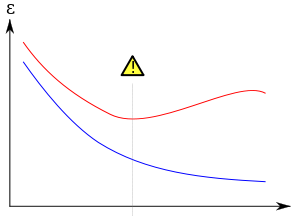
\includegraphics[width=0.5\textwidth]{figure/ann/overfitting}
    \caption{A toy example of overfitting. The red line shows the error on the validation data and the blue line shows the error on the training data. It is desired that the error is as low as possible. 
    "\href{https://en.wikipedia.org/wiki/Overfitting\#/media/File:Overfitting_svg.svg}{Overfitting}" by
    \href{https://commons.wikimedia.org/wiki/User:Gringer}{Gringer} edited by
    \href{https://commons.wikimedia.org/wiki/User\:Dake}{Dake} is licensed under CC-BY 3.0.}
    \label{fig:overfitting}
\end{figure}
\\
As seen in Figure \ref{fig:overfitting} the network is performing better and better for both training and validation sets. However, it reaches a point where the validation error starts going up. That point is where the overfitting has occurred. The training error is still decreasing meaning that the network keeps learning on the training data instead of generalising from it. 

\subsection{Regularisation}\label{sec:regularisation}
Regularisation is a set of techniques used in order to prevent the overfitting problem described in section \ref{sec:overfitting}. These techniques increase the performance of the network as it can continue to generalise without overfitting. 
In this thesis two different regularisation techniques have been used:
\begin{itemize}
    \item Dropout
    \item L2-loss
\end{itemize}
These will be thoroughly explained below.
\\\\
\textbf{Dropout} is a rather newly discovered regularisation technique that prevents overfitting by randomly disabling neurons in the ANN \parencite{srivastava2014dropout}. During the training of the network, neurons are randomly disabled with a probability $p$. This means that the network has to teach other neurons to do the generalisation that the disabled neuron previously did. It is important to note that this is only used during the training of the network. When validating the performance of the network or actually using the network all neurons are used.
\\\\
The purpose of \textbf{L2-loss regularisation} is to prevent weights from becoming extremely large by penalising them based on how large they are, this leads to a limitation in capacity i.e. that not all functions can be approximated. The L2 regularisation is used by adding the L2-norm of every weight in the ANN to the error function.
\\\\

A powerful aspect of these two regularisation techniques is that they work alongside each other. This is because they are implemented in different parts of the ANN model.

\section{Recurrent Neural Networks (RNN)}\label{sec:rnn}
A recurrent neural network is an artificial neural network that takes context into account. It accounts for context in the sense that the current output is dependent on the previous. This context dependency is often depicted as an ANN that has its own output as input, in practice however RNNs are instead modelled as chained (or \textit{unfolded}) \textit{units} as shown in Figure \ref{fig:chained_units}. A unit takes two inputs; the output from the previous unit and input data. The output produced is passed along to the next unit but could also be retrieved and used. An arbitrary number of units can be chained in this way but in this project the number of units will be related to the length of the input text. 
\begin{figure}[h]
    \centering
    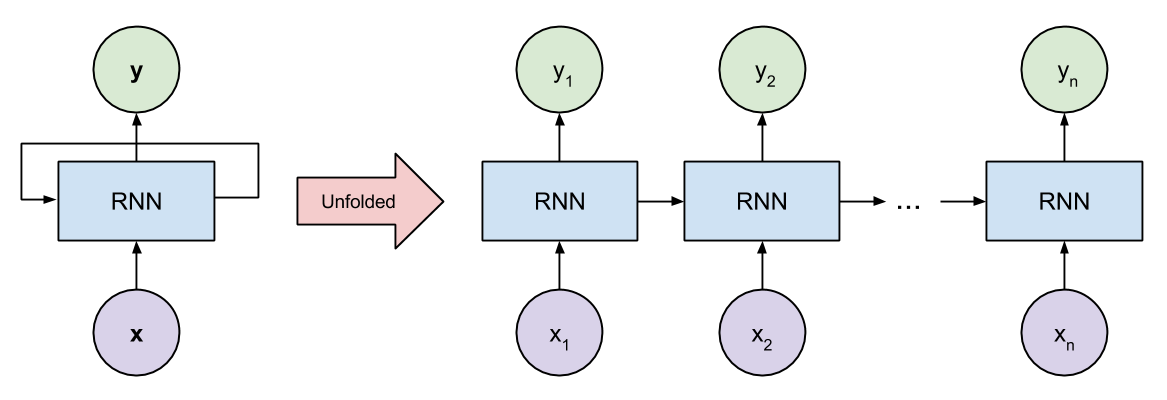
\includegraphics[width=0.95\textwidth]{figure/ann/rnn_unfold}
    \caption{A visualisation of a recurrent neural network layer and how it is unfolded. $\vec{x}$ and $\vec{y}$ are the input and output vector respectively}
    \label{fig:chained_units}
\end{figure}
\\
RNNs are particularly useful when modelling with natural language as input since words in a sentence often are dependent on what comes before them. When using sentences as input to a RNN, it is common to have each word as an input to one unit in the RNN \parencite{palangi2016deep}. This is how RNNs will be used in this project to model social platform content.
\\\\
The units in a recurrent neural network can be implemented in different ways. Popular unit implementations are Long Short Term Memory (LSTM) and Gated Recurrent Unit (GRU). The LSTM unit was introduced to solve the problems of inefficiency in the backpropagation for RNNs \parencite{LSTMdefined}. The inefficiencies occurred because the error gradient would decay and approach zero, making training very slow, and this is what the LSTM solves \parencite{hochreiter1998vanishing}. The GRU is a fairly recent addition to the field of RNN. It performs similarly to the LSTM and the dataset used can have a big impact on which one performs better \parencite{GRUchung2014empirical}. The fact that either of the unit implementations might perform better based on the dataset used motivates testing them both in this project.

\subsection{Using RNNs for NLP}\label{sec:rnn_nlp}
As previously mentioned, when working with natural language it is common to let every unit in a RNN layer take one word as input. This is illustrated in figure \ref{fig:sentence_to_rnn} below.
\begin{figure}[h]
    \centering
    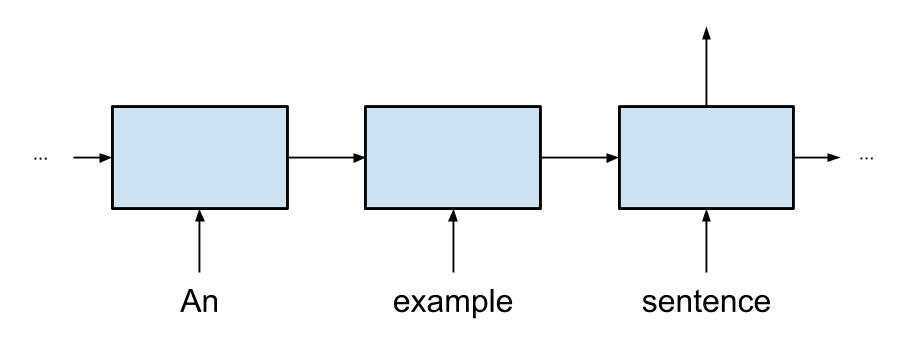
\includegraphics[width=0.75\textwidth]{figure/ann/sentence_to_rnn}
    \caption{A simplification of how a recurrent neural network layers process natural language as input}
    \label{fig:sentence_to_rnn}
\end{figure}
\\
However, RNN units, just as an ANN, expect some vector. This means that the input sentences have to be vectorised. A common way to achieve this is to use indices instead. With this approach each unique word is given a unique number, and an input sentence of words then become a vector of word indices. It is also common to take the transformation one step further and turn each word index into a so called one-hot vector \parencite{turian2010word}. Using one-hot vectors, each word is represented as a vector $\vec{w}$ of length $C$, where $C$ represents the total number of words, having a $1$ at the position of the given word's index and zeros everywhere else, this is illustrated by the table \ref{tab:onehot}. Since the length of the vector is fixed, it means that the new words that are not in the dictionary can not be represented as a one-hot vector. 
\begin{table}[h]
    \centering
    \begin{tabular}{c|c|c|c|c}
    This & is & a & normal & sentence\\
    \hline
    1 & 0 & 0 & 0 & 0\\
    0 & 1 & 0 & 0 & 0\\
    0 & 0 & 1 & 0 & 0\\
    0 & 0 & 0 & 1 & 0\\
    0 & 0 & 0 & 0 & 1
    \end{tabular}
    \caption{An illustration of how the sentence "This is a normal sentence" as one-hot vectors, given that the vocabulary is \{a, is, normal, sentence, this\}}
    \label{tab:onehot}
\end{table} 
\\\\
Another problem with one-hot vectors is that they do not hold any information about relationships between words. This motivates using another representation for words in order to capture the connection. This can be done with algorithms such as word2vec \parencite{mikolov2013linguistic} or GloVe \parencite{pennington2014glove}. 